
%%%%%%%%%%%%%%%%%%%%%%%%%%%%%%%%%%%%%%%%%%%%%%%%%%%%%%%%%%%%%%%%%%%

\newcommand{\XXX}[1]{\textcolor{red}{#1}}
\newcommand{\system}[1]{\textsc{#1}}

\frame{\frametitle{Tuning task}

\begin{itemize}
\item So many things to choose in tuning (metric, algorithm, data, features...)
\pause \item Final performance usually measured by BLEU and not humans
\pause \item Organised Tuning Task on WMT15 to explore these options in proper way
\end{itemize}
}

\frame{\frametitle{Tuning task - system for tuning}

\begin{itemize}
\item Hiero Moses trained both for English-Czech and Czech-English on small dataset
\pause \item constrained version allowed 2000 sentence pairs for tuning
\pause \item constrained version allowed only dense features
\pause \item any tuning algorithm or metric tuning was allowed (even manually setting weights)
\end{itemize}
}

% \frame{\frametitle{Data}
%     \begin{table}[t]
%     \centering
%     \tiny
%     \begin{tabular}{llcc|cc|cc}
%     %           & Source & \begin{tabular}[c]{@{}l@{}}en-cs\\ \#sents\end{tabular} & \begin{tabular}[c]{@{}l@{}}cs-en \\ \#sents\end{tabular} & Tokens \\
%     		   &        & \multicolumn{2}{c|}{Sentences} & \multicolumn{2}{c|}{Tokens} & \multicolumn{2}{c}{Types} \\
%     		   & Source & cs & en & cs & en & cs & en \\
%     \hline
%     LM corpora &  News Commentary v8      &  162309  & 247966    &  3.6M & 6.2M & 162K & 81K  \\
%     TM corpora &  Europarl v7, CCrawl and News Comm. v9 &  \multicolumn{2}{c|}{911952} & 17.7M & 20.8M & 652K & 361K \\
%     Dev set &  newstest2014 &  \multicolumn{2}{c|}{3003}    & 51K & 60K & 19K & 13K        \\
%     Test set &  newstest2015 &  \multicolumn{2}{c|}{2656}   & 39K & 47K & 16K & 11K      \\
%     \end{tabular}
%     \caption{Data used in the WMT15 tuning task.}
%     \label{table:data}
%     \end{table}
% } 

% \frame{\frametitle{OOV words}
%     \begin{table}[t]
%     \centering
%     \small
%     \begin{tabular}{crr|rr}
%      & \multicolumn{2}{c|}{Dev} & \multicolumn{2}{c}{Test} \\
%     Direction & Token & Type & Token & Type \\ \hline
%     en-cs & 2570 & 2032 & 2003 & 1655 \\
%     cs-en & 3891 & 3415 & 3381 & 3011 \\
%     \end{tabular}
%     \caption{Out of vocabulary word counts}
%     \label{table:oov}
%     \end{table}
% }

\frame{\frametitle{Czech-English results}
    
\begin{table}
\begin{center}
\small
\begin{tabular}{rrr|r}
\textbf{System Name}   & \multicolumn{2}{c|}{\textbf{TrueSkill Score}} & \textbf{BLEU}\\
                       & \llap{Tun}ing-Only & All & \\
\hline
% \system{bleu-MIRA-dense	} & 0.3869 \\ \hline
% \system{AFRL		        } & 0.3824 \\ \hline
% \system{ILLC-UvA		} & 0.3740 \\ \hline
% \system{USAAR-Tuna	} & 0.3699 \\ \hline
% \system{bleu-MERT-dense		} & 0.3654 \\ \hline
% \system{DCU		        } & 0.3600 \\ \hline
% \system{METEOR-CMU		} & 0.3304 \\ \hline
% \system{bleu-MIRA-sparse	} & 0.3198 \\ \hline
% \system{HKUST			} & 0.3113 \\ \hline

\system{bleu-MIRA-dense		} & 0.153   & -0.182 & 12.28 \\
\system{ILLC-UvA		} & 0.108       & -0.189 & 12.05 \\
\system{bleu-MERT-dense		} & 0.087   & -0.196 & 12.11 \\
\system{AFRL		        } & 0.070   & -0.210 & 12.20 \\
% cluster border in tuning-only
\cline{2-2}
\system{USAAR-Tuna	} & 0.011       & -0.220 & 12.16 \\
\cline{3-3} % cluster border in all
\system{DCU		        } & -0.027  & -0.263 & 11.44 \\
% cluster border                           & \\
\cline{2-2} % \specialrule{.3em}{.2em}{.2em}
\system{METEOR-CMU		} & -0.101     & -0.297 & 10.88 \\
\system{bleu-MIRA-sparse	} & -0.150 & -0.320 & 10.84 \\
\system{HKUST			} & -0.150     & -0.320 & 10.99 \\ 
\hline
% \cline{1-2} % \specialrule{.3em}{.2em}{.2em}
\system{HKUST-LATE		} & --- & --- & 12.20 \\
\end{tabular}
\caption{Results on Czech-English tuning}
\label{table:results-csen}
\end{center}
\end{table}

} 

\frame{\frametitle{English-Czech results}
    
\begin{table}
%\begin{center}
\small
\hspace{-5mm}
\begin{tabular}{rrr|r}
\textbf{System Name}   & \multicolumn{2}{c|}{\textbf{TrueSkill Score}} & \textbf{BLEU}\\
                       & \llap{Tun}ing-Only & All & \\
\hline

\system{DCU			} & 0.320  & -0.342 & 4.96 \\
\system{bleu-MIRA-dense		} & 0.303  & -0.346 & 5.31 \\
\system{AFRL			} & 0.303  & -0.342 & 5.34 \\
\cline{2-3} % \specialrule{.3em}{.2em}{.2em}
\system{USAAR-Tuna	} & 0.214  & -0.373 & 5.26 \\
\cline{2-3} % \specialrule{.3em}{.2em}{.2em}
\system{bleu-MERT-dense		} & 0.123  & -0.406 & 5.24 \\
\cline{2-3} % \specialrule{.3em}{.2em}{.2em}
\system{METEOR-CMU		} & -0.271 & -0.563 & 4.37 \\
\cline{2-3} % \specialrule{.3em}{.2em}{.2em}
\system{bleu-MIRA-sparse	} & -0.992 & -0.808 & 3.79 \\ \hline
\system{USAAR-baseline-mira	} & ---   & ---  & 5.31 \\
\system{USAAR-baseline-mert	} & ---  & ---   & 5.25 \\


% \system{DCU			} & 0.3198 \\ \hline	
% \system{AFRL			} & 0.3151 \\ \hline			
% \system{bleu-MIRA-dense		} & 0.3071 \\ \hline
% \system{USAAR-Tuna	} & 0.2833 \\ \hline	
% \system{bleu-MERT-dense		} & 0.2659 \\ \hline
% \system{METEOR-CMU		} & 0.2544 \\ \hline
% \system{bleu-MIRA-sparse	} & 0.1767 \\ \hline
\end{tabular}
\caption{Results on English-Czech tuning}
\label{table:results-encs}
%\end{center}
\end{table}

} 

\frame{\frametitle{Word Penalty weights for English-Czech}
    %\begin{figure}[t]
    \begin{center}
    {
    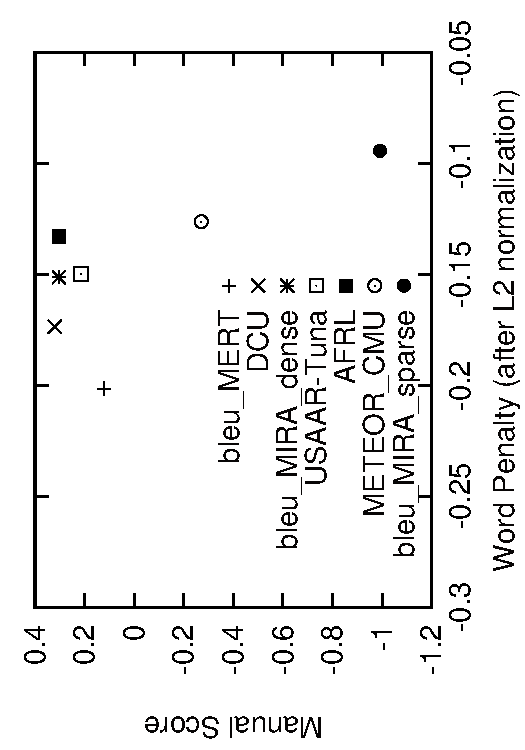
\includegraphics[width=0.6\columnwidth,angle=270]{wpplotL2.pdf}
    }
    \end{center}
    % \caption{Relation between the word penalty and the final performance of systems
    % translating from English to Czech.}
    % \label{wpplot}
    % \end{figure}
    \begin{itemize}
	\item Difficult to analyse individual weights but if we have to...
	\item All non-sparse systems find similar weights for WP
    \end{itemize}
} 

\frame{\frametitle{English-Czech PCA}
%        \begin{tabular}{cc}
    %\begin{figure}[t]
    \begin{center}
    %\vspace{-7mm}
    {
    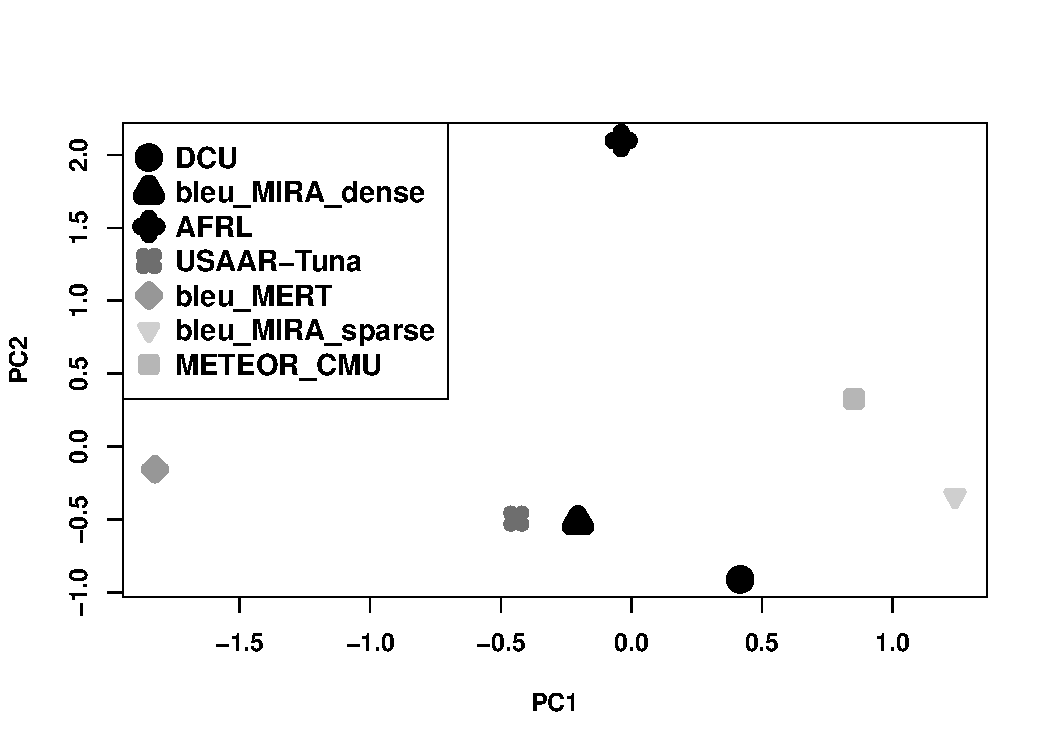
\includegraphics[width=0.99\columnwidth]{en-cs_PCA.pdf}
    }
    \end{center}
    %\caption{PCA for English-Czech. The darker the point, the higher the manual
    %score.}
    %\label{pca_encs}
    %\end{figure}
%	&
%    \begin{table}
%      \small
%      \begin{center}
%        \begin{tabular}{l|r|r}
%    
%                         &   PC1 &   PC2 \\\hline
%    LM0                  & \textbf{-0.69} &  0.44 \\
%    PhrasePenalty0       &  0.15 & \textbf{-0.63} \\
%    TranslationModel0\_0 & \textbf{-0.91} & -0.13 \\
%    TranslationModel0\_1 & \textbf{ 0.91} & -0.03 \\
%    TranslationModel0\_2 & -0.55 &  \textbf{0.72} \\
%    TranslationModel0\_3 &  0.36 &  \textbf{0.75} \\
%    TranslationModel1    &  0.42 &  \textbf{0.84} \\
%    WordPenalty0         & \textbf{ 0.84} &  0.27 \\
%        \end{tabular}
%    \caption{Loadings (correlations) of each component with each feature function for English-Czech}
%    \label{pca_loadings}
%      \end{center}
%    \end{table}
%\\ \end{tabular}
}

\frame{\frametitle{Table of contents}
    \begin{table}
      \small
      \begin{center}
        \begin{tabular}{l|r|r}
    
                         &   PC1 &   PC2 \\\hline
    LM0                  & \textbf{-0.69} &  0.44 \\
    PhrasePenalty0       &  0.15 & \textbf{-0.63} \\
    TranslationModel0\_0 & \textbf{-0.91} & -0.13 \\
    TranslationModel0\_1 & \textbf{ 0.91} & -0.03 \\
    TranslationModel0\_2 & -0.55 &  \textbf{0.72} \\
    TranslationModel0\_3 &  0.36 &  \textbf{0.75} \\
    TranslationModel1    &  0.42 &  \textbf{0.84} \\
    WordPenalty0         & \textbf{ 0.84} &  0.27 \\
        \end{tabular}
    \caption{Loadings (correlations) of each component with each feature function for English-Czech}
    \label{pca_loadings}
      \end{center}
    \end{table}
}

\frame{\frametitle{Czech-English PCA}
    
    %\begin{figure}[t]
    \begin{center}
    \vspace{-7mm}
    {
    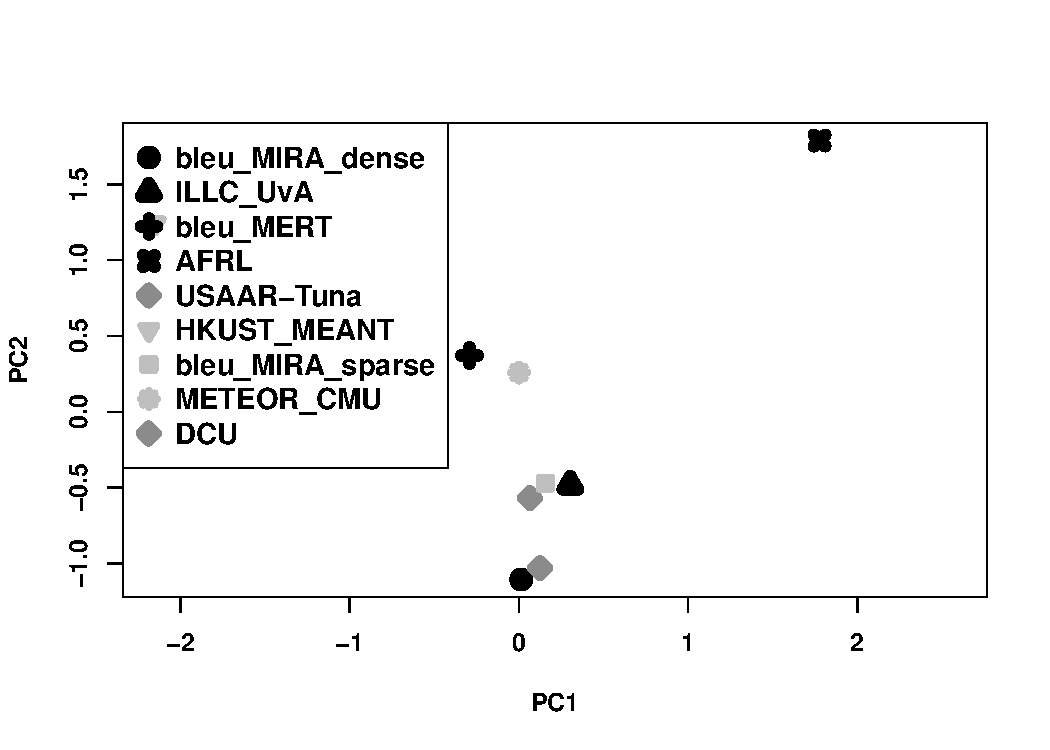
\includegraphics[width=0.90\columnwidth]{cs-en_PCA.pdf}
    }
    \end{center}
    %\caption{PCA for Czech-English. The darker the point, the higher the manual
    %score.}
    %\label{pca_csen}
    %\end{figure}
	\begin{itemize}
		\item No obvious pattern
		\item Very similar systems perform complitely differently
		\item Very different systems perform similarly
	\end{itemize}

} 
